\chapter{Architecture}

\begin{figure}
	\centering
	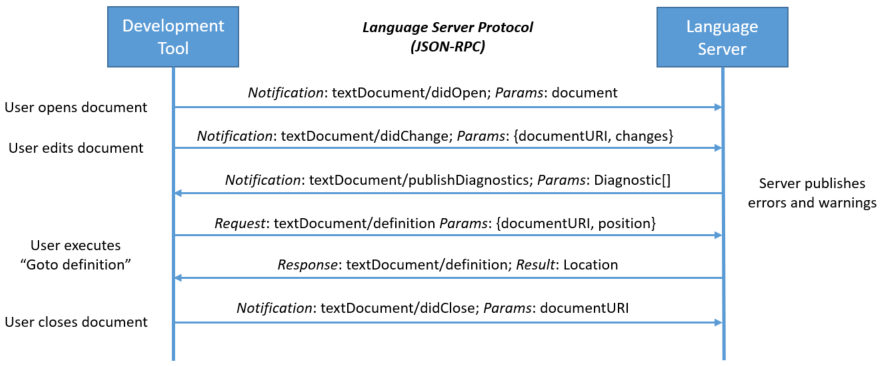
\includegraphics[width=\textwidth]{img/language-server-sequence}
	\caption[LSP session example.]{LSP session example. (source: LSP overview)}
	\label{fig04:LSP}
	\small\textsuperscript{https://microsoft.github.io/language-server-protocol/}
\end{figure}

\begin{figure}
	\centering
	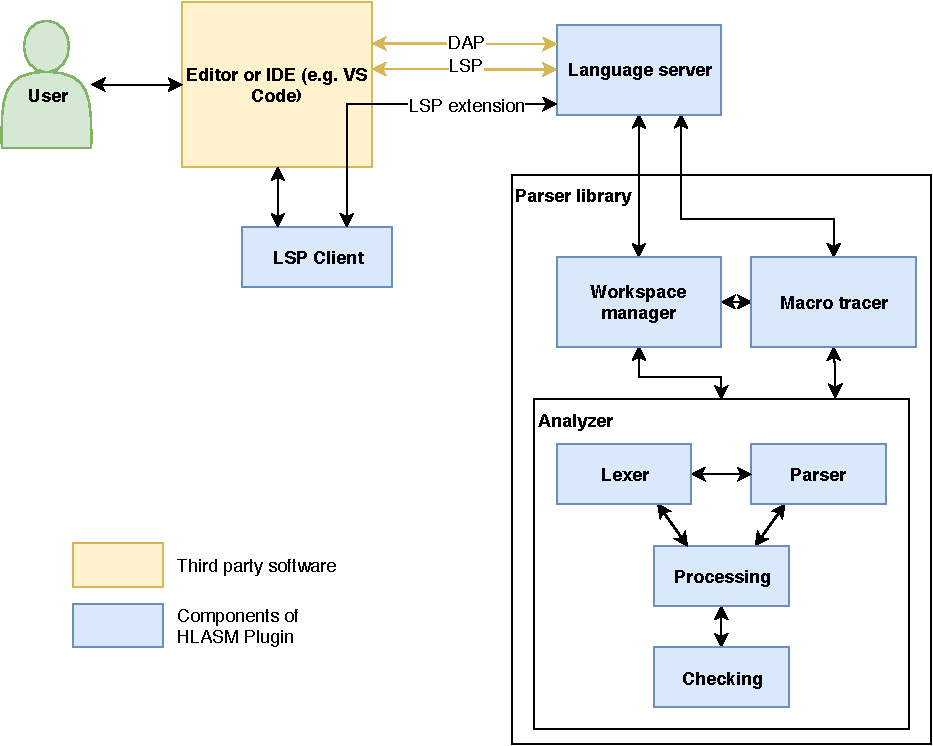
\includegraphics[width=\textwidth]{img/hlasm_architecture}
	\caption{The architecture of HLASM Plugin}
	\label{fig04:arch}
\end{figure}

The architecture is based on the way modern code editors and IDEs are extended to support additional languages. We chose to implement Language Server Protocol \footnote{\label{note1}https://microsoft.github.io/language-server-protocol/} (LSP), which is supported by a majority of contemporary editors.

In LSP, the two parties that communicate are called a \emph{client} and a\emph{language server}. A simple example is displayed in Figure~\cref{fig04:LSP} The client runs as a part of an editor. The language server may be a standalone application that is connected to the client by a pipe or TCP. All language-specific user actions are transformed into standard LSP messages and sent to the language server. The language server then analyzes the source code and sends back a response, which is then interpreted and presented to the user in editor-specific way. This architecture makes possible to only have one LSP client implementation for each code editor, which may be reused by all programming languages. And vice versa, every language server may be easily used by any editor that has an implementation of the LSP client.

To add support for HLASM, we have to implement the LSP language server and write a thin extension to an editor, which will use an already existing implementation of the LSP client. To implement source code highlighting, we need to extend the protocol with a new notification. This notification will be used for transferring information from language server to VS Code client, which is extended to highlight code in editor based on the incoming custom notifications.

This chapter presents the decomposition of the project into smaller components and describes their relations. The two main components are the parser library and the language server --- an executable application that uses the parser library. The overall architecture is pictured in Figure~\cref{fig04:arch}.

\section{Language server}

The responsibility of the Language server component is to maintain the LSP session, convert incoming JSON messages and use the parser library to execute them. The functionality includes:
\begin{itemize}
    \item reading LSP messages from standard input or TCP and writing responses
    \item parsing JSON RPC to C++ structures, so they can be further used
    \item serializing C++ structures into JSON, so it can be sent back to the client
    \item implementing asynchronous request handling: e.g. when user makes several consecutive changes to a source code, it is not needed to parse on every change
\end{itemize}

\section{Parser library}

Parser library is the core of the project --- it encapsulates all parsing capabilities, keeps track of open files in the editor and provides information about them. Its API is based on LSP --- every relevant request and notification has a corresponding method in the parsing library. The API includes:

\begin{itemize}
	\item Implementation of text synchronization notifications (didOpen, didChange, didClose), which inform the library about files that are currently open in the editor and their exact contents.
	\item Implementation of workspace management notifications (DidChangeWorkspaceFolders): many editors have capabilities to open more workspaces at the same time, and the parser library supports this too. Workspace is basically just a folder which contains related source codes. Workspaces help parser library find macro and copy files.
	\item A method to consume DidChangeWatchedFiles notification. This method makes it possible to react to workspace changes that were not made by the user in editor, but may still affect the parsing. For example, when a user deletes an external macro file, the parser library should react by reporting that it cannot find the macro.
	\item Implementation of diagnostics publishing (publishDiagnostics notification). A diagnostic is used to indicate a problem with source files, such as a compiler error or a warning. The parser library provides a callback to let the language server know that diagnostics have changed.
	\item Callback for highlighting information provision.
	\item Implementation of language feature requests (definition, references, hover, completion), which provide information needed for proper reaction of the editor on user actions.
	
\end{itemize}

The parser library is further decomposed into smaller components.

\subsection{Analyzer}

The analyzer is able to process a single HLASM file. The processing includes:
\begin{itemize}
 \item recognition of statements and their parts (lexing and parsing)
 \item interpretation of instructions that should be executed in compile time
 \item a check whether the HLASM source code is well-formed
 \item reporting of problems with the source by producing LSP diagnostics
 \item providing highlighting and LSP information
\end{itemize}

A HLASM file may have dependencies --- other files that define macros or files brought in by the COPY instruction. The dependencies are only discovered during the processing of files, so it is not possible to provide the files beforehand. The analyzer must get a callback that would find a file with specified name, parse its contents and return it as list of parsed statements. 

To sum up, the analyzer has a pretty simple API: it takes the contents of a source file by common string and a callback that can parse external files with specified name. It provides a list of diagnostics linked to the file, highlighting, list of symbol definitions, etc.

The analyzer is further decomposed into 4 components.

\subsubsection{Lexer}

Lexer's task is to read source string and break it into tokens --- small pieces of text with special meaning. The most important properties of the lexer:
\begin{itemize}
	\item each token has location in the source text
	\item has the ability to check whether all characters are valid in the HLASM source
	\item has the ability to jump in the source file backward and forward if necessary (for implementation of instructions like AGO and AIF)
\end{itemize}

Because of the specificity of HLASM language the lexer is implemented from scratch since we found it hard to use lexing tools.

\subsubsection{Parser}

Parser component takes the stream of tokens the lexer produces and recognizes HLASM statements according to syntax. To accomplish this, a parser generator tool Antlr 4 \footnote{https://www.antlr.org} is used.

The input to Antlr is a grammar (written in antlr-specific language) that specifies the syntax of HLASM language and generates source code (in C++) for a recognizer, which is able to tell whether input source code is valid or not. Moreover, it is possible to assign a piece of code that executes every time a grammar rule is matched by the recognizer to further process the matched piece of code.


\subsubsection{Processing}

Results of the parser component are further analyzed in the processing component. Its most important capabilities are:
\begin{itemize}
	\item Interpretation of CA instructions, which results in modifying the lexer state (moving back and forth in the input file).
	\item Substitution of variable symbols. After the substitution, the statement must be reparsed in the lexer and the parser.
	\item Interpretation of assembler instructions to evaluate ordinary symbols.
	\item MACRO and COPY expansion.
\end{itemize}

\subsubsection{Checking}
After a statement is fully processed and all operands of each instruction are known, the statement needs to be checked for errors. There are over 2000 machine instructions with variable number of operands and various restrictions on those operands --- some of them take only positive numbers, numbers that are in specific range or are limited to addresses only. The checking component takes an instruction and list of its operands and returns a list of warnings or error in a form of LSP diagnostics.

\subsection{Workspace manager}

The responsibility of a workspace manager is to keep the representation of workspaces and files in the parser library exactly the same as the user sees in the editor. Further, it starts the analyzer when needed, manages workspace configuration and provides external macro and copy libraries to analyzer.

\section{VS code extension}

The VS Code extension component ensures seamless integration with the editor. Its functions are:

\begin{itemize}
	\item to start the HLASM language server and the LSP client that comes with VS Code, and create a connection between them
	\item to implement server-side highlighting, which extends the LSP protocol
	\item to improve user experience regarding continuations and fixed length line source codes
\end{itemize}


\section{Macro tracer}
A macro tracer enables the user to trace the compilation of HLASM source code in a way similar to common debugging. This is the reason why we chose to implement a Debug Adapter Protocol \footnote{https://microsoft.github.io/debug-adapter-protocol/} (DAP). It is very similar to LSP, so most of the code implementing LSP in the language server component may be reused for both protocols.

The language server component communicates with the macro tracer component in the parser library. Its API mirrors the requests and events of DAP. The most important features to implement are:

\begin{itemize}
	\item launch, continue, next, stepIn and disconnect requests, which allow user to control the flow of the compilation
	\item SetBreakpoints, which get information about breakpoints that the user has placed in the code
	\item Threads, StackTrace, Scopes and Variables requests to allow the DAP client to retrieve information about the current processing stack (stack of nested macros and copy instructions), available variable symbols and their values
	\item stopped, exited and terminated events to let the DAP client know about state of traced source code
\end{itemize}

The macro tracer communicates with the workspace manager to retrieve the content of the traced files. Afterwards, it starts analyzing the source file in a separate thread and gets callbacks from the analyzer before a statement is processed. In the callback, the tracer puts the thread to sleep and waits for user interaction. During this time, it is possible to retrieve all variable and stack information from the processing to display it to the user.
